\section{Connection}

\subsection{Connection message system}

Beskeder i systemet foregår via en række objekter, der alle nedarver fra en basis klasse ved navn Message. Disse er beskrevet nærmere i følgende afsnit

\subsubsection{Message}
Indeholder en enum af typen MessageTypes, hvori alle typer beskeder fremgår. Desuden indeholder den en string med MessageInfo, som primært anvendes i tilfælde af fejl, hvor beskeden vises i systemets GUI som vist på figur~\ref{fig:loginError}

\begin{figure}
	\centering
	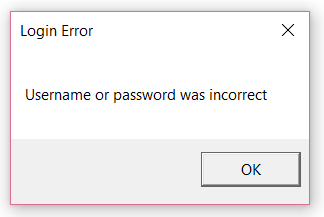
\includegraphics[width=0.3\linewidth]{figs/connection/loginError.png}
	\caption{Login error}
	\label{fig:loginError}
\end{figure}

\subsubsection{ClientMsg}
Indeholder ikke yderligere informationer, men definerer en adskillelse mellem server beskeder og klient beskeder. Desuden giver det mulighed for at alle klient beskeder i fremtiden kan indeholder informationer, som server beskeder ikke indeholder. 

\paragraph{ResetPasswordRequestMsg}
Denne beskedtype er ikke blevet færdigt implementeret. Beskeden var tiltænkt at skulle sende en mail til brugeren med et nyt password, men blev nedprioriteret pga. tidsmangel.
\begin{lstlisting}[caption=ResetPasswordRequestMsg, label=code:ResetPasswordRequestMsg]
public class ResetPasswordRequestMsg : ClientMsg
{
	public string Username { get; set; }
	
	public ResetPasswordRequestMsg(string username)
	{
		Username = username;
		MsgType = MessageTypes.ResetPasswordRequest;
	}
}
\end{lstlisting}

\paragraph{AddUserRequestMsg}
Indeholder de informationer der bliver gemt i databasen når en bruger bliver oprettet.
\begin{lstlisting}[caption=AddUserRequestMsg, label=code:AddUserRequestMsg]
public class AddUserRequestMsg : ClientMsg
{
	public string Fullname { get; set; }
	public string Username { get; set; }
	public string Password { get; set; }
	
	public AddUserRequestMsg(string fullname, string username, string password)
	{
		Fullname = fullname;
		Username = username;
		Password = password;
		MsgType = MessageTypes.AddUserRequest;
	}
}
\end{lstlisting}

\paragraph{LoginRequestMsg}
Indeholder informationer til at kontrollere om brugeren har indtastet det korrekte password
\begin{lstlisting}[caption=LoginRequestMsg, label=code:LoginRequestMsg]
public class LoginRequestMsg : ClientMsg
{
	public string Username { get; set; }
	public string Password { get; set; }
	
	public LoginRequestMsg(string username, string password)
	{
		Username = username;
		Password = password;
		MsgType = MessageTypes.LoginRequest;
	}
}
\end{lstlisting}

\subsubsection{TokenMsg}
Alle beskedtyper som kræver at brugeren er logget ind, nedarver fra denne besked. Beskeden indeholder udover en MsgType også en SubMsgType, til at definere hvilken nedarving af TokenMsg der er tale om. Dette er lavet så alle nedarvinger beholder typen TokenMsg som deres MsgType.
\begin{lstlisting}[caption=TokenMsg, label=code:TokenMsg]
public class TokenMsg : ClientMsg
{
	public string Username { get; set; }
	public string TokenString { get; set; }
	public TokenSubMessageTypes SubMsgType { get; set; }
	
	public TokenMsg(string username, string tokenString)
	{
		Username = username;
		TokenString = tokenString;
		MsgType = MessageTypes.TokenMsg;
	}
}
\end{lstlisting}

\paragraph{AddPoolRequest}
Indeholder informationer til at beskrive brugerens pool i systemet.
\begin{lstlisting}[caption=AddPoolRequest, label=code:AddPoolRequest]
public class AddPoolRequestMsg : TokenMsg
{
	public string PoolName { get; set; }
	public double Volume { get; set; }
	public string SerialNumber { get; set; }
	
	public AddPoolRequestMsg(string username, string tokenString, string poolName, double poolVolume, string serialNumber) : base(username, tokenString)
	{
		PoolName = poolName;
		Volume = poolVolume;
		SerialNumber = serialNumber;
		SubMsgType = TokenSubMessageTypes.AddPoolRequest;
	}
}
\end{lstlisting}

\paragraph{GetPoolDataRequest}
Indeholder informationer om hvilke data der ønskes modtaget i klienten. Beskeden kan oprettes med propperty GetAllNamesOnly sat til true, hvis klienten kun ønsker at modtage en liste med navne over alle pools brugeren har tilknyttet. Denne liste vil yderligere indeholde en bool for hver pool, som er true hvis en eller flere måleværdier er udenfor deres target værdi. En anden mulighed at angive et pool navn, hvilket resulterer i et svar med informationer om konkrete målinger, indenfor en tidsperiode der svarer til det angivne antal dage.
\begin{lstlisting}[caption=GetPoolDataRequest, label=code:GetPoolDataRequest]
public class GetPoolDataRequestMsg : TokenMsg
{
	public bool GetAllNamesOnly { get; set; }
	public string PoolName { get; set; }
	public int GetHistoryDays { get; set; }
	
	public GetPoolDataRequestMsg(string username, string tokenString, bool getAllNamesOnly = false, string poolName = "", int getHistoryDays = 0)
	: base(username, tokenString)
	{
		GetAllNamesOnly = getAllNamesOnly;
		PoolName = poolName;
		GetHistoryDays = getHistoryDays;
		SubMsgType = TokenSubMessageTypes.GetPoolDataRequest;
	}
}
\end{lstlisting}

\paragraph{GetPoolInfoRequest}
Indeholder navnet på den pool der ønskes information om, så som pool volume og serial number.
\begin{lstlisting}[caption=GetPoolInfoRequest, label=code:GetPoolInfoRequest]
public class GetPoolInfoRequestMsg : TokenMsg
{
	public string PoolName { get; set; }
	
	public GetPoolInfoRequestMsg(string username, string tokenString, string poolName) : base(username, tokenString)
	{
		PoolName = poolName;
		SubMsgType = TokenSubMessageTypes.GetPoolInfoRequest;
	}
}
\end{lstlisting}

\paragraph{RemovePoolRequest}
Indeholder navnet på den pool, brugeren ønsker at fjerne.
\begin{lstlisting}[caption=RemovePoolRequest, label=code:RemovePoolRequest]
public class RemovePoolRequestMsg : TokenMsg
{
	public string PoolName { get; set; }
	
	public RemovePoolRequestMsg(string username, string tokenString, string poolName) : base(username, tokenString)
	{
		PoolName = poolName;
		SubMsgType = TokenSubMessageTypes.RemovePoolRequest;
	}
}
\end{lstlisting}

\paragraph{UpdatePoolRequest}
Indeholder informationer som giver brugeren mulighed for at ændre en pools navn eller volume.
\begin{lstlisting}[caption=UpdatePoolRequest, label=code:UpdatePoolRequest]
public class UpdatePoolRequestMsg : TokenMsg
{
	public string OldPoolName { get; set; }
	public string NewPoolName { get; set; }
	public double NewPoolVolume { get; set; }
	
	public UpdatePoolRequestMsg(string username, string tokenString, string oldPoolName, string newPoolName = "", double newPoolVolume = 0) : base(username, tokenString)
	{
		OldPoolName = oldPoolName;
		NewPoolName = newPoolName;
		NewPoolVolume = newPoolVolume;
		SubMsgType = TokenSubMessageTypes.UpdatePoolRequest;
	}
}
\end{lstlisting}

\paragraph{ChangePasswordRequest}
Indholder informationer om brugerens gamle password, samt hvilket password brugeren fremover ønsker at benytte.
\begin{lstlisting}[caption=ChangePasswordRequest, label=code:ChangePasswordRequest]
public class ChangePasswordRequestMsg : TokenMsg
{
	public string OldPassword { get; set; }
	public string NewPassword { get; set; }
	
	public ChangePasswordRequestMsg(string username, string tokenString, string oldPassword, string newPassword) : base(username, tokenString)
	{
		OldPassword = oldPassword;
		NewPassword = newPassword;
		SubMsgType = TokenSubMessageTypes.ChangePasswordRequest;
	}
}
\end{lstlisting}

\paragraph{LogoutRequest}
Indeholder ikke yderligere informationer, da klassen allerede nedarver fra TokenMsg og dermed har username som en del af beskeden.
\begin{lstlisting}[caption=LogoutRequest, label=code:LogoutRequest]
public class LogoutRequestMsg : TokenMsg
{
	public LogoutRequestMsg(string username, string tokenString) : base(username, tokenString)
	{
		SubMsgType = TokenSubMessageTypes.LogoutRequest;
	}
}
\end{lstlisting}

\subsubsection{ServerMsg}
Denne klasse indeholder ikke yderligere informationer, men definerer en række beskeder som serveren kan svare med. Det er forsøgt at holde antallet af beskeder så lavt som muligt, ved f.eks. at lave en GeneralResponseMsg som anvendes på alle requests, hvor applikationen ikke modtager data, men blot ønsker at vide om den pågældende request blev udført. 

\paragraph{GeneralResponseMsg}
Indeholder informationer om hvor vidt en request blev udført. Der gives yderligere information om det skyldes at brugerens session ikke længere er aktiv, eller at det var selve requesten der fejlede.
\begin{lstlisting}[caption=GeneralResponseMsg, label=code:GeneralResponseMsg]
public class GeneralResponseMsg : ServerMsg
{
	public bool TokenStillActive { get; set; }
	public bool RequestExecutedSuccesfully { get; set; }
	public GeneralResponseMsg(bool tokenStillActive, bool requestExecutedSuccesfully)
	{
		TokenStillActive = tokenStillActive;
		RequestExecutedSuccesfully = requestExecutedSuccesfully;
		MsgType = MessageTypes.GeneralResponse;
	}
}
\end{lstlisting}

\paragraph{GetPoolDataResponse}
Indeholder enten informationer om alle poolnavne til en bruger, eller sensor målinger for en enkelt pool.
\begin{lstlisting}[caption=GetPoolDataResponse, label=code:GetPoolDataResponse]
public class GetPoolDataResponseMsg : ServerMsg
{
	public List<Tuple<SensorTypes, List<double>>> SensorList { get; set; }
	public List<Tuple<string, bool>> AllPoolNamesListTuple { get; set; }
	
	public GetPoolDataResponseMsg(List<Tuple<SensorTypes, List<double>>> sensorList = null, List<Tuple<string, bool>> allPoolNamesListTuple = null )
	{
		SensorList = sensorList;
		AllPoolNamesListTuple = allPoolNamesListTuple;
		MsgType = MessageTypes.GetPoolDataResponse;
	}
}
\end{lstlisting}

\paragraph{GetPoolInfoResponse}
Indeholder informationer om en brugers pool
\begin{lstlisting}[caption=GetPoolInfoResponse, label=code:GetPoolInfoResponse]
public class GetPoolInfoResponseMsg : ServerMsg
{
	public double Volume { get; set; }
	public string SerialNumber { get; set; }
	
	public GetPoolInfoResponseMsg(double volume, string serialNumber)
	{
		Volume = volume;
		SerialNumber = serialNumber;
		MsgType = MessageTypes.GetPoolInfoResponse;
	}
}
\end{lstlisting}

\paragraph{LoginResponse}
Indeholder informationer om hvor vidt det lykkedes at logge ind på systemet. Hvis login lykkedes, vil beskeden også indeholde en TokenString, som applikationen derefter sender med fremtidige requests.
\begin{lstlisting}[caption=LoginResponse, label=code:LoginResponse]
public class LoginResponseMsg : ServerMsg
{
	public string TokenString { get; set; }
	public bool LoginSuccessful { get; set; }
	
	public LoginResponseMsg(string tokenString, bool loginSuccessful)
	{
		TokenString = tokenString;
		LoginSuccessful = loginSuccessful;
		MsgType = MessageTypes.LoginResponse;
	}
}
\end{lstlisting}

\subsection{Client}
I denne sektion er beskrevet hvorledes klienten er opbygget. Klienten står for at modtage besked objekter fra applikations laget, og omsætte disse til strings der kan sendes til serveren. Desuden står klienten for at modtage svar fra serveren, og omdanne disse til den korrekte beskedtype. 

\subsubsection{Synchronous Socket Client}
Er den konkrete implementering af socket client, som anvendes med en windows desktop applikation. Klassen er implementeret udfra eksemplet fundet på https://msdn.microsoft.com/en-us/library/kb5kfec7(v=vs.110).aspx ?? . Der er tilføjet exception handling, i tilfælde af at serveren ikke svarer. Andre konkrete klienter er baseret på samme princip.

\subsubsection{ClientMessenger}
Modtager et besked objekt fra applikations laget. Dette bliver serializeret til en string vha. Json. Der anvendes JsonSettings da det er nedarvede objekter som serializeres, og der derfor er behov for flere oplysninger om objektet, end hvad der som standard genereres med Json. Derefter sendes beskeden vha. en IClient og en IClientReponseManager håndterer svaret før det returneres til applikations laget. Dette ses af koden i figur ??
\begin{lstlisting}[caption=Client.SendMessage, label=code:Client.SendMessage]
public Message SendMessage(Message message)
{
	return _clientResponseManager.HandleMessage(_client.StartClient(JsonConvert.SerializeObject(message, _jsonSettings) + "<EOF>"));
}
\end{lstlisting}

\subsubsection{Client Response Manager}
Modtager en string som indeholder informationer om et objekt. Ved først at deserializere objektet til basis klassen message, oprettes en switch case på beskedens type som vist på figur ??
\begin{lstlisting}[caption=Client.HandleMessage, label=code:Client.HandleMessage]
public Message HandleMessage(string messageString)
{
	var receivedMessage = JsonConvert.DeserializeObject<Message>(messageString);
	
	switch (receivedMessage.MsgType)
	{
		case MessageTypes.LoginResponse:
		return JsonConvert.DeserializeObject<LoginResponseMsg>(messageString);
		
		case MessageTypes.GeneralResponse:
		return JsonConvert.DeserializeObject<GeneralResponseMsg>(messageString);
		
		case MessageTypes.GetPoolDataResponse:
		return JsonConvert.DeserializeObject<GetPoolDataResponseMsg>(messageString);
		
		case MessageTypes.GetPoolInfoResponse:
		return JsonConvert.DeserializeObject<GetPoolInfoResponseMsg>(messageString);
		
		default:
		if (receivedMessage.MessageInfo != null)
			return new Message(receivedMessage.MessageInfo);
		else
		{
			return new Message("An unknown error occured");
		}
	}
}
\end{lstlisting}

\subsection{Server}
I denne sektion er beskrevet hvorledes serveren er opbygget. Serveren står for at modtage strings, omdanne dem til besked objekter og lave tilsvarende kald til databasen efter behov. Desuden simuleres pool data i serveren, og der holdes styr på user sessions vha. en TokenKeeper. 

\subsubsection{Asynchronous Socket Listener}
Den primære funktionalitet af denne klasse er hentet fra https://msdn.microsoft.com/en-us/library/fx6588te(v=vs.110).aspx ?? . Denne fungerer ved at køre asynchront, hvilket vil sige at applikationen ikke idler når der afventes en connection. Dette vil med andre ord sige, at der kan oprettes flere forbindelser til serveren på samme tid, da de ikke blokkerer hinanden.
Der er ændret i klassens konsol output, så essentielle data vises. Dette kan ses på figur~\ref{fig:asynchronousSocketListener}

\begin{figure}
	\centering
	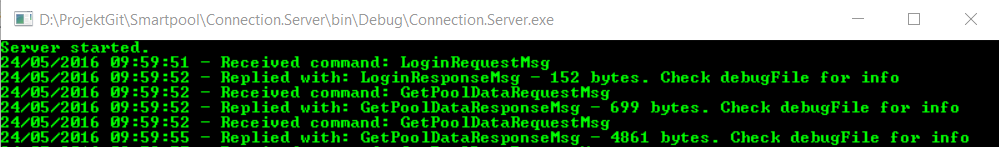
\includegraphics[width=0.9\linewidth]{figs/connection/asynchronousSocketListener.png}
	\caption{Asynchronous Socket Listener}
	\label{fig:asynchronousSocketListener}
\end{figure}

Udfra de viste informationer kan man hurtigt se hvilken type besked der er modtaget, samt hvilken type besked der er svaret med, samt hvor meget denne besked fylder. Det fulde output bliver desuden gemt i en log fil, så det efterfølgende er muligt at se præcis hvilke informationer der er sendt. Dette er valgt for at gøre server vinduet overskueligt, uden at miste essentielle informationer.

Der er desuden valgt at lade exceptions blive vist i server vinduet, som f.eks. ses på figur~\ref{fig:asynchronousSocketListenerException} hvor databasen har genereret en exception, da der er forsøgt at lave et login med et ukendt brugernavn.

\begin{figure}
	\centering
	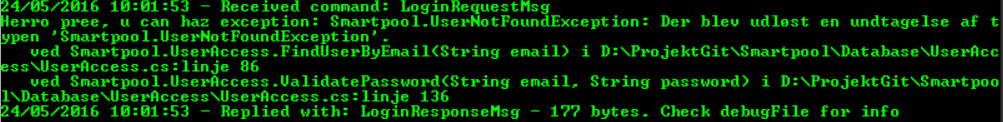
\includegraphics[width=0.9\linewidth]{figs/connection/asynchronousSocketListenerException.png}
	\caption{Asynchronous Socket Listener Exception}
	\label{fig:asynchronousSocketListenerException}
\end{figure}

Som det også fremgår i server vinduet figur~\ref{fig:asynchronousSocketListenerException} bliver en exception håndteret af serveren, og der sendes en besked af den korrekte type tilbage til klient applikationen, så hverken server eller klient crasher.

\subsubsection{Response Manager}
Denne klasse er primært baseret på en switch case, hvor der baseret på den modtagne beskeds type, returneres et passende svar som set på figur ??
\begin{lstlisting}[caption=Server.ResponseManager, label=code:Server.ResponseManager]
var receivedMessage = JsonConvert.DeserializeObject<Message>(receivedString, _jsonSettings);

switch (receivedMessage.MsgType)
{
	case MessageTypes.LoginRequest:
	var loginMessage = JsonConvert.DeserializeObject<LoginRequestMsg>(receivedString);
	return HandleLoginRequest(loginMessage);
	
	case MessageTypes.TokenMsg:
	var tokenMessage = JsonConvert.DeserializeObject<TokenMsg>(receivedString);
	if (_tokenKeeper.TokenActive(tokenMessage.Username, tokenMessage.TokenString))
		return _tokenMsgResponse.HandleTokenMsg(receivedMessage, receivedString, _tokenKeeper);
	else return new GeneralResponseMsg(false, false);
	
	case MessageTypes.AddUserRequest:
	var addUserMessage = JsonConvert.DeserializeObject<AddUserRequestMsg>(receivedString);
	return new GeneralResponseMsg(false, _smartpoolDb.UserAccess.AddUser(addUserMessage.Fullname, addUserMessage.Username, addUserMessage.Password));
	
	case MessageTypes.ResetPasswordRequest:
	var resetPasswordMessage = JsonConvert.DeserializeObject<ResetPasswordRequestMsg>(receivedString);
	return new GeneralResponseMsg(false, false);
	
	default:
	return new GeneralResponseMsg(false, false)	{MessageInfo = "The server did not recognize your request"};
}
\end{lstlisting}

Klassens switch-case er indkapslet i en try block, hvori der sørges for at eventuelle exceptions bliver håndteret, og der sendes et passende svar tilbage til klienten. Der er yderligere lavet en metode til håndtering af login requests, da denne som den eneste krævede en længere håndtering. Denne anvender en task til at kalde i databasen, da dette ved test af og til tog længere tid end forventet. Metoden ses på figur ??

\begin{lstlisting}[caption=Server.ResponseManager.HandleLoginRequest, label=code:Server.ResponseManager.HandleLoginRequest]
var task = Task.Run(() => _smartpoolDb.UserAccess.ValidatePassword(loginMsg.Username, loginMsg.Password));
if (task.Wait(TimeSpan.FromSeconds(15))) //if task is completed within time limit
{
	return task.Result ? new LoginResponseMsg(_tokenKeeper.CreateNewToken(loginMsg.Username), true) : new LoginResponseMsg("", false) {MessageInfo = "Username or password was incorrect"};
}
else
	return new LoginResponseMsg("", false) {MessageInfo = "Login timed out. Please try again later"};
\end{lstlisting}

\subsubsection{Token System}
Oprettelse af nye tokens sker ved at kalde metoden CreateNewToken med et username som parameter. Dette username bliver gemt i et token objekt, som også indeholder en token string genereret af TokenStringGenerator, samt en DateTime variabel. DateTime variablen indeholder oplysninger om hvornår denne token sidst blev anvendt/oprettet.
For at undgå at inactive tokens bliver liggende i systemet, sørger TokenKeeper for at tælle en variabel ned, som definerer hvornår den skal rydde op i sin liste af aktive tokens. Til sidst returnerer TokenKeeper den genererede TokenString, som bliver sendt tilbage til klient applikationen. Det hele ses på~\ref{code:ServerTokenKeeperCreateNewToken}
\begin{lstlisting}[caption=Server.TokenKeeper.CreateNewToken, label=code:ServerTokenKeeperCreateNewToken]
public string CreateNewToken(string username)
{
	var newToken = new Token(username, _tokenStringGenerator, _tokenLifeTime);
	_tokens.Add(newToken);
	
	if (_removeUnusedCountdown == 0)
	{
		RemoveAllUnusedTokens();
		_removeUnusedCountdown = _tokensCreatedBeforeRemovingUnused;
	}
	_removeUnusedCountdown--;
	
	return newToken.GetTokenString();
}
\end{lstlisting}

\subsubsection{Pool DataGeneration}
\paragraph{PoolKeeper} er implementeret som en fake klasse, der indeholder en liste over pools i systemet. Ved opstart chekkes på få udvalgte brugernavne i databasen, som der derefter genereres tilsvarende pools for. Desuden bliver der, mens systemet kører, oprettet pools i systemet for nye pools der tilføjes til databasen. Så længe serveren kører, vil alle nye pools altså generere data.

\paragraph{Pool} er implementeret som en fake klasse. Klassen indeholder ikke nogen public metoder, da den er selvkørende og ved et angivet interval selv opretter sensor data i databasen. Dette er tiltænkt at være tilsvarende et reelt system, hvor en reel pool klasse, ved et givet interval, sender en request til en fysisk enhed om måledata, som derefter gemmes i databasen.

Oprettelse af en pool via klassens constructor ses på ??
\begin{lstlisting}[caption=Server.FakePool.Constructor, label=code:ServerFakePoolConstructor]
public Pool(int secondsBetweenSensorReadings, string userName, string poolName, ISmartpoolDB smartpoolDb)
{
	UserName = userName;
	PoolName = poolName;
	SmartpoolDb = smartpoolDb;
	_fakeSensors = new List<ISensor>();
	GenerateSensors();
	var timer = new Timer { Interval = 1000 * secondsBetweenSensorReadings };
	timer.Elapsed += SaveSensorValue;
	timer.Start();
}
\end{lstlisting}

\paragraph{Sensor} er implementeret som en fake klasse. Der er lagt stor vægt på at klassen genererer værdier som kunne være reele, da dette er med til at give et helhedsindtryk af det endelige system. 

\paragraph{SensorValueAuthenticator} som et led i at give sensoren realistiske værdier, er denne klasse oprettet for at angive en minimum og maximum værdi, en given sensor type kan have.